%%%%%%%%%%%%%%%%%%%%%%%%%%%%%%%%%%%%%%%%%%%%%%%%%%%%%%%%%%%%%%%%%%%%%%%%%%%%%%%
% Grupo 1 - Atividades de Ensino
%%%%%%%%%%%%%%%%%%%%%%%%%%%%%%%%%%%%%%%%%%%%%%%%%%%%%%%%%%%%%%%%%%%%%%%%%%%%%%%

%%%%%%%%%%%%%%%%%%%%%%%%%%%%%%%%%%%%%%%%%%%%%%%%%%%%%%%%%%%%%%%%%%%%%%%%%%%%%%%
% Subgrupo 1.1 - Orientações e Co-Orientações
%%%%%%%%%%%%%%%%%%%%%%%%%%%%%%%%%%%%%%%%%%%%%%%%%%%%%%%%%%%%%%%%%%%%%%%%%%%%%%%

\newpage
\subsection{Orientação de Teses de Doutorado Concluídas}
\label{advisor:phd-concluidas}
Esta subseção apresenta o comprovante de orientações de Tese de Doutorado concluídas.
\includepdf[pages=-, scale=1,pagecommand=\thispagestyle{empty}]{\detokenize{GRUPO 1/Sub-Grupo 11/Comprovante Fake}}

\newpage
\subsection{Co-Orientação de Teses de Doutorado Concluídas}
\label{co-advisor:phd-concluidas}
Esta subseção apresenta o comprovante de co-orientações de Tese de Doutorado concluídas.
\includepdf[pages=-, scale=1,pagecommand=\thispagestyle{empty}]{\detokenize{GRUPO 1/Sub-Grupo 11/Comprovante Fake}}

\newpage
\subsection{Orientação de Teses de Doutorado em Andamento}
\label{advisor:phd-andamento}
Esta subseção apresenta o comprovante de orientações de Tese de Doutorado em andamento.
\includepdf[pages=-, scale=1,pagecommand=\thispagestyle{empty}]{\detokenize{GRUPO 1/Sub-Grupo 11/Comprovante Fake}}

\newpage
\subsection{Co-Orientação de Teses de Doutorado em Andamento}
\label{co-advisor:phd-andamento}
Esta subseção apresenta o comprovante de co-orientações de Tese de Doutorado em andamento.
\includepdf[pages=-, scale=1,pagecommand=\thispagestyle{empty}]{\detokenize{GRUPO 1/Sub-Grupo 11/Comprovante Fake}}

\newpage
\subsection{Orientação de Dissertações de Mestrado Concluídas}
\label{advisor:msc-concluidas}
Esta subseção apresenta o comprovante de orientações de Dissertação de Mestrado concluídas.
\includepdf[pages=-, scale=1,pagecommand=\thispagestyle{empty}]{\detokenize{GRUPO 1/Sub-Grupo 11/Comprovante Fake}}

\newpage
\subsection{Co-Orientação de Dissertações de Mestrado Concluídas}
\label{co-advisor:msc-concluidas}
Esta subseção apresenta o comprovante de co-orientações de Dissertação de Mestrado concluídas.
\includepdf[pages=-, scale=1,pagecommand=\thispagestyle{empty}]{\detokenize{GRUPO 1/Sub-Grupo 11/Comprovante Fake}}

\newpage
\subsection{Orientação de Dissertações de Mestrado em Andamento}
\label{advisor:msc-andamento}
Esta subseção apresenta o comprovante de orientações de Dissertação de Mestrado em andamento.
\includepdf[pages=-, scale=1, pagecommand=\thispagestyle{empty}]{\detokenize{GRUPO 1/Sub-Grupo 11/Comprovante Fake}}

\newpage
\subsection{Co-Orientação de Dissertações de Mestrado em Andamento}
\label{co-advisor:msc-andamento}
Esta subseção apresenta o comprovante de co-orientações de Dissertação de Mestrado em andamento.
\includepdf[pages=-, scale=1,pagecommand=\thispagestyle{empty}]{\detokenize{GRUPO 1/Sub-Grupo 11/Comprovante Fake}}

\newpage
\subsection{Orientação de Dissertação de Mestrado Profissional Conluídas}
\label{advisor:mprof-concluidas}
Esta subseção apresenta o comprovante de orientações de Dissertação de Mestrado Profissional concluídas.
\includepdf[pages=-, scale=1,pagecommand=\thispagestyle{empty}]{\detokenize{GRUPO 1/Sub-Grupo 11/Comprovante Fake}}

\newpage
\subsection{Co-Orientação de Dissertação de Mestrado Profissional Conluídas}
\label{co-advisor:mprof-concluidas}
Esta subseção apresenta o comprovante de co-orientações de Dissertação de Mestrado Profissional concluídas.
\includepdf[pages=-, scale=1,pagecommand=\thispagestyle{empty}]{\detokenize{GRUPO 1/Sub-Grupo 11/Comprovante Fake}}

\newpage
\subsection{Orientações de Mestrado Profissional em Andamento}
\label{advisor:mprof-andamento}
Esta subseção apresenta o comprovante de orientações de Dissertação de Mestrado Profissional em andamento.
\includepdf[pages=-, scale=1,pagecommand=\thispagestyle{empty}]{\detokenize{GRUPO 1/Sub-Grupo 11/Comprovante Fake}}

\newpage
\subsection{Co-Orientações de Mestrado Profissional em Andamento}
\label{co-advisor:mprof-andamento}
Esta subseção apresenta o comprovante de co-orientações de Dissertação de Mestrado Profissional em andamento.
\includepdf[pages=-, scale=1,pagecommand=\thispagestyle{empty}]{\detokenize{GRUPO 1/Sub-Grupo 11/Comprovante Fake}}

\newpage
\subsection{Orientações de Trabalhos de Conclusão de Curso Concluídas}
\label{advisor:tcc}
Esta subseção apresenta o comprovante de orientações de Trabalhos de Conclusão de Curso concluídas.
\includepdf[pages=-, scale=1,pagecommand=\thispagestyle{empty}]{\detokenize{GRUPO 1/Sub-Grupo 11/Comprovante Fake}}

\newpage
\subsection{Orientações de Monitorias}
\label{advisor:monitoria}
Esta subseção apresenta o comprovante de orientações de Monitoria no período de 2014-2 a 2016-1 impressa diretamente da página do Sistema de Gerenciamento de Monitores Online (GMon)\footnote{URL: \url{https://www.cin.ufpe.br/~gmon}, Último acesso em XX/XX/XXXX}.
\includepdf[pages=-, scale=1,pagecommand=\thispagestyle{empty}]{\detokenize{GRUPO 1/Sub-Grupo 11/Comprovante Fake}}

\newpage
\subsection{Orientações de Trabalhos de Apoio Acadêmico}
\label{advisor:icc}
Esta subseção apresenta o comprovante de orientações de Trabalhos de Iniciação Científica.
\includepdf[pages=-, scale=1,pagecommand=\thispagestyle{empty}]{\detokenize{GRUPO 1/Sub-Grupo 11/Comprovante Fake}}

\newpage
\subsection{Orientações de Trabalhos de Apoio Acadêmico}
\label{advisor:bia}
Esta subseção apresenta o comprovante de orientações de Trabalhos de Apoio Acadêmico.
\includepdf[pages=-, scale=1,pagecommand=\thispagestyle{empty}]{\detokenize{GRUPO 1/Sub-Grupo 11/Comprovante Fake}}


%%%%%%%%%%%%%%%%%%%%%%%%%%%%%%%%%%%%%%%%%%%%%%%%%%%%%%%%%%%%%%%%%%%%%%%%%%%%%%%
% Subgrupo 1.2 - Participação em Comiss\~{o}es Examinadoras
%%%%%%%%%%%%%%%%%%%%%%%%%%%%%%%%%%%%%%%%%%%%%%%%%%%%%%%%%%%%%%%%%%%%%%%%%%%%%%%

\newpage
\subsection{Parecerista dos cursos de Sistemas de Informação da Avaliação de Cursos Superiores do Guia do Estudante (GE) 2015}
\label{app:2015-guia-estudante}
Esta subseção apresenta o comprovante da atuação como parecerista dos cursos de Sistemas de Informação da Avaliação de Cursos Superiores do Guia do Estudante (GE) 2015, promovido pela Editora Abril.
\includepdf[pages=-, scale=1,pagecommand=\thispagestyle{empty}]{\detokenize{GRUPO 1/Sub-Grupo 12/1/Comprovante Fake}}

%---

\newpage
\subsection{Comissão Avaliadora dos trabalhos na área de Ciências Exatas apresentados na 19ª Jornada de Iniciação Científica da FACEPE}
\label{app:2015-jic-facepe}
Esta subseção apresenta o comprovante da atuação como Membro da Comissão Avaliadora dos trabalhos na área de Ciências Exatas apresentados na 19ª Jornada de Iniciação Científica da Fundação de Amparo a Ciência e Tecnologia do Estado de Pernambuco (FACEPE).
\includepdf[pages=-, scale=1,pagecommand=\thispagestyle{empty}]{\detokenize{GRUPO 1/Sub-Grupo 12/2/Comprovante Fake}}

%---

\newpage
\subsection{Participação em Bancas de Trabalho de Conclusão de Curso}
\label{app:bancas-tcc}
Esta subseção apresenta o comprovante da atuação membro nas Bancas Examinadoras de Trabalho de Conclusão de Curso no Centro de Informática/UFPE.
\includepdf[pages=-, scale=1,pagecommand=\thispagestyle{empty}]{\detokenize{GRUPO 1/Sub-Grupo 12/4/Comprovante Fake}}

\newpage
\subsection{Participação em Banca de Dissertação }
\label{app:2015-msc-hslb}
Esta subseção apresenta o comprovante da atuação membro na Banca Examinadora de Defesa de Dissertação de Mestrado de 
\includepdf[pages=-, scale=1,pagecommand=\thispagestyle{empty}]{\detokenize{GRUPO 1/Sub-Grupo 12/5/Comprovante Fake}}

%---

\newpage
\subsection{Participação em Banca de Qualifica\c{c}\~ao / Proposta de Tese de Doutorado}
\label{app:2015-quali-phd-tmp}
Esta subseção apresenta o comprovante da atuação como membro na Banca Examinadora de Defesa de Proposta de Tese de Doutorado 
\includepdf[pages=-, scale=1,pagecommand=\thispagestyle{empty}]{\detokenize{GRUPO 1/Sub-Grupo 12/6/Comprovante Fake}}

%---

\newpage
\subsection{Participação em Banca de Tese de Doutorado }
\label{app:2015-phd-jcd}
Esta subseção apresenta o comprovante da atuação como membro na Banca Examinadora de Defesa de Tese de Doutorado 
\includepdf[pages=-, scale=1,pagecommand=\thispagestyle{empty}]{\detokenize{GRUPO 1/Sub-Grupo 12/7/Comprovante Fake}}

%---

\newpage
\subsection{Participação como Membro Externo da Comissão de Seleção para o Doutorado }
\label{app:2015-pgcomp-pdse}
Esta subseção apresenta o comprovante da atuação como membro Externo da Comissão de Seleção para o Doutorado 
\includepdf[pages=-, scale=1,pagecommand=\thispagestyle{empty}]{\detokenize{GRUPO 1/Sub-Grupo 12/8/Comprovante Fake}}

%%%%%%%%%%%%%%%%%%%%%%%%%%%%%%%%%%%%%%%%%%%%%%%%%%%%%%%%%%%%%%%%%%%%%%%%%%%%%%%
% Subgrupo 1.3 - Atividades de Ensino na Graduação e na Pós-Graduação
%%%%%%%%%%%%%%%%%%%%%%%%%%%%%%%%%%%%%%%%%%%%%%%%%%%%%%%%%%%%%%%%%%%%%%%%%%%%%%%



%%%%%%%%%%%%%%%%%%%%%%%%%%%%%%%%%%%%%%%%%%%%%%%%%%%%%%%%%%%%%%%%%%%%%%%%%%%%%%%
% Subgrupo 1.4 - Avaliação Didática Docente pelo Discente
%%%%%%%%%%%%%%%%%%%%%%%%%%%%%%%%%%%%%%%%%%%%%%%%%%%%%%%%%%%%%%%%%%%%%%%%%%%%%%%

\newpage
\subsection{Avaliação Didática Docente pelo Discente}
\label{evaluation:2015-1}
Esta subseção apresenta o comprovante da Avaliação Didática Docente pelo Discente para o período do primeiro semestre de 2015.
\includepdf[pages=-, scale=1,pagecommand=\thispagestyle{empty}]{\detokenize{GRUPO 1/Sub-Grupo 14/Comprovante Fake}}

%%%%%%%%%%%%%%%%%%%%%%%%%%%%%%%%%%%%%%%%%%%%%%%%%%%%%%%%%%%%%%%%%%%%%%%%%%%%%%%
% Subgrupo 2.1 - Produtividade de Pesquisa
%%%%%%%%%%%%%%%%%%%%%%%%%%%%%%%%%%%%%%%%%%%%%%%%%%%%%%%%%%%%%%%%%%%%%%%%%%%%%%%

\newpage
\subsection{Bolsista de produtividade em pesquisa e em inovação tecnolÓgica}
\label{app:bolsista-prod}
Esta subseção apresenta o comprovante de Bolsista de produtividade em pesquisa e em inovação tecnolÓgica.
\includepdf[pages=-, scale=1,pagecommand=\thispagestyle{empty}]{\detokenize{GRUPO 2/Sub-Grupo 21/A/Comprovante Fake}}

\newpage
\subsection{Participação em Eventos Científicos (com apresentação de trabalho ou oferecimento de cursos, palestras ou debates}
\label{app:2015-cbsoft}
Esta subseção apresenta o comprovante da participação no Congresso Brasileiro de Software: Teoria e Prática (CBSoft'2015) com seus respectivos propósitos.
\includepdf[pages=-, scale=1,pagecommand=\thispagestyle{empty}]{\detokenize{GRUPO 2/Sub-Grupo 21/B/Comprovante Fake}}

\newpage
\subsection{Participação em Eventos Científicos (com apresentação de trabalho ou oferecimento de cursos, palestras ou debates}
\label{app:2015-enacomp}
Esta subseção apresenta o comprovante da participação no XII Encontro Anual de Computação (EnAComp) com seus respectivos propósitos.
\includepdf[pages=-, scale=1,pagecommand=\thispagestyle{empty}]{\detokenize{GRUPO 2/Sub-Grupo 21/B/Comprovante Fake}}
\includepdf[pages=-, scale=1,pagecommand=\thispagestyle{empty}]{\detokenize{GRUPO 2/Sub-Grupo 21/B/Comprovante Fake}}
\includepdf[pages=-, scale=1,pagecommand=\thispagestyle{empty}]{\detokenize{GRUPO 2/Sub-Grupo 21/B/Comprovante Fake}}

%---

\newpage
\subsection{Autoria de artigos completos publicados em anais de congresso, em jornais e revistas de circulação nacional e internacional na sua área}
\label{conf:2015-sbcup}
Esta subseção apresenta o comprovante da autoria de artigo completo publicado em anais do 7º Simpósio Brasileiro de Computação Ubíqua e Pervasiva (SBCUP)\footnote{\url{http://csbc2015.cin.ufpe.br/eventos_descricao/13}}, Evento do XXXV Congresso da Sociedade Brasileira de Computação.
\includepdf[pages=-, scale=1,pagecommand=\thispagestyle{empty}]{\detokenize{GRUPO 2/Sub-Grupo 21/C/Comprovante Fake}}

%---

\newpage
\subsection{Arbitragem de Artigos Técnico-Científicos Nacionais e Internacionais na sua área de atuação}
\label{reviewer:2015-tsc}
Esta subseção apresenta o comprovante de arbitragem de artigos do periódico IEEE Transactions on Services Computing, editora IEEE Computer Society, ISSN: 1939-1374.
\includepdf[pages=-, scale=1,pagecommand=\thispagestyle{empty}]{\detokenize{GRUPO 2/Sub-Grupo 21/D/Comprovante Fake}}

%---

\newpage
\subsection{Coordenação e/ou Participação em Projetos Aprovados por Órgãos de Fomento}
\label{project:2015-facepe-pepe}
Esta subseção apresenta o comprovante de coordenação e/ou participação no Projeto \textit{``BIGStore - Evolução da plataforma Ustore para Armazenamento, Manipulação e Experimentação de Grandes Volumes de Dados''} aprovado pela Fundação de Amparo à Ciência e Tecnologia do Estado de Pernambuco (FACEPE), Edital FACEPE 23/2014 - PESQUISADOR NA EMPRESA DE PERNAMBUCO (PEPE).
\includepdf[pages=-, scale=1,pagecommand=\thispagestyle{empty}]{\detokenize{GRUPO 2/Sub-Grupo 21/E/Comprovante Fake}}

%---

\newpage
\subsection{Consultoria às Instituições de Fomento à Pesquisa, Ensino e Extensão}
\label{consulting:2015-facepe-pepe}
Esta subseção apresenta o comprovante de consultoria à Fundação de Amparo à Ciência e Tecnologia do Estado de Pernambuco (FACEPE) no Seminário de Avaliação Final dos Projetos Aprovados no Edital 10.2/2012 - PAPPE INTEGRAÇÃO 04a RODADA.
\includepdf[pages=-, scale=1,pagecommand=\thispagestyle{empty}]{\detokenize{GRUPO 2/Sub-Grupo 21/F/Comprovante Fake}}

%---

\newpage
\subsection{Prêmios Recebidos pela Produção Científica e Técnica}
\label{award:2014}
Esta subseção apresenta o comprovante de consultoria à Fundação de Amparo à Ciência e Tecnologia do Estado de Pernambuco (FACEPE) no Seminário de Avaliação Final dos Projetos Aprovados no Edital 10.2/2012 - PAPPE INTEGRAÇÃO 04a RODADA.
\includepdf[pages=-, scale=1,pagecommand=\thispagestyle{empty}]{\detokenize{GRUPO 2/Sub-Grupo 21/G/Comprovante Fake}}

%%%%%%%%%%%%%%%%%%%%%%%%%%%%%%%%%%%%%%%%%%%%%%%%%%%%%%%%%%%%%%%%%%%%%%%%%%%%%%%
% Subgrupo 2.2 - Produção Científica
%%%%%%%%%%%%%%%%%%%%%%%%%%%%%%%%%%%%%%%%%%%%%%%%%%%%%%%%%%%%%%%%%%%%%%%%%%%%%%%

\newpage
\subsection{Trabalhos Publicados em PeriÓdicos Especializados do País ou do Exterior}
\label{journal:2015-medinfo}
Esta subseção apresenta o comprovante de publicação do artigo ```(Br-SCMM) Brazilian Smart City Maturity Model: A Perspective from the Health Domain'' no Studies in Health Technology and Informatics, v. 216 (MEDINFO 2015: eHealth-enabled Health), p. 983, 2015, doi: 10.3233/978-1-61499-564-7-983.
\includepdf[pages=-, scale=1,pagecommand=\thispagestyle{empty}]{\detokenize{GRUPO 2/Sub-Grupo 22/Comprovante Fake}}

%%%%%%%%%%%%%%%%%%%%%%%%%%%%%%%%%%%%%%%%%%%%%%%%%%%%%%%%%%%%%%%%%%%%%%%%%%%%%%%
% Grupo 3: Atividades de Extensão
%%%%%%%%%%%%%%%%%%%%%%%%%%%%%%%%%%%%%%%%%%%%%%%%%%%%%%%%%%%%%%%%%%%%%%%%%%%%%%%

%%%%%%%%%%%%%%%%%%%%%%%%%%%%%%%%%%%%%%%%%%%%%%%%%%%%%%%%%%%%%%%%%%%%%%%%%%%%%%%
% Subgrupo 3.1 - Coordenação e Orientação
%%%%%%%%%%%%%%%%%%%%%%%%%%%%%%%%%%%%%%%%%%%%%%%%%%%%%%%%%%%%%%%%%%%%%%%%%%%%%%%

\newpage
\subsection{Coordenação e Orientação de Atividades de Extensão}
\label{extensao:2015}
Esta subseção apresenta o comprovante de Coordenação e Orientação de Atividades de Extensão.
\includepdf[pages=-, scale=1,pagecommand=\thispagestyle{empty}]{\detokenize{GRUPO 3/Sub-Grupo 31/Comprovante Fake}}

%%%%%%%%%%%%%%%%%%%%%%%%%%%%%%%%%%%%%%%%%%%%%%%%%%%%%%%%%%%%%%%%%%%%%%%%%%%%%%%
% Subgrupo 3.2 - Coordenação de Eventos e Conferencista
%%%%%%%%%%%%%%%%%%%%%%%%%%%%%%%%%%%%%%%%%%%%%%%%%%%%%%%%%%%%%%%%%%%%%%%%%%%%%%%

\newpage
\subsection{Comissão Organizadora de Eventos Internacional, Nacional, Regional ou Local}
\label{reviewer:2015-sbcars}
Esta subseção apresenta o comprovante de Comissão Organizadora do 9th Brazilian Symposium on Software Components, Architectures and Reuse (SBCARS 2015).
\includepdf[pages=-, scale=1,pagecommand=\thispagestyle{empty}]{\detokenize{GRUPO 3/Sub-Grupo 32/Comprovante Fake}}

%%%%%%%%%%%%%%%%%%%%%%%%%%%%%%%%%%%%%%%%%%%%%%%%%%%%%%%%%%%%%%%%%%%%%%%%%%%%%%%
% Grupo 4: Atividades de Formação e Capacitação Acadêmica
%%%%%%%%%%%%%%%%%%%%%%%%%%%%%%%%%%%%%%%%%%%%%%%%%%%%%%%%%%%%%%%%%%%%%%%%%%%%%%%

\newpage
\subsection{Atualização e Cursos de Capacitação ou Extensão na área de Conhecimento ou Afins com no Mínimo 40h}
\label{courses:2015}
Esta subseção apresenta o comprovante de Atualização e Cursos de Capacitação ou Extensão no curso Machine Learning (Coursera).
\includepdf[pages=-, scale=1,pagecommand=\thispagestyle{empty}]{\detokenize{GRUPO 4/Comprovante Fake}}

%%%%%%%%%%%%%%%%%%%%%%%%%%%%%%%%%%%%%%%%%%%%%%%%%%%%%%%%%%%%%%%%%%%%%%%%%%%%%%%
% Grupo 5: Atividades Administrativas
%%%%%%%%%%%%%%%%%%%%%%%%%%%%%%%%%%%%%%%%%%%%%%%%%%%%%%%%%%%%%%%%%%%%%%%%%%%%%%%

\newpage
\subsection{Atividades Administrativas, Membro de Comissão Temporária}
\label{committee:temp-2015}
Esta subseção apresenta o comprovante de Atividades Administrativas, Membro de Comissão Temporária.
\includepdf[pages=-, scale=1,pagecommand=\thispagestyle{empty}]{\detokenize{GRUPO 5/Comprovante Fake}}

%------------------------------------------------------------------------------

\newpage
\subsection{Atividades Administrativas, Coordenador de Curso Pós-Graduação \textbf{strictu sensu}}
\label{committee:postgrad-2015}
Esta subseção apresenta o comprovante de Atividades Administrativas, Coordenador de Curso Pós-Graduação \textbf{strictu sensu}.
\includepdf[pages=-, scale=1,pagecommand=\thispagestyle{empty}]{\detokenize{GRUPO 5/Comprovante Fake}}

%------------------------------------------------------------------------------

\newpage
\subsection{Atividades Administrativas, Membro de Núcleo Docente Estruturante}
\label{committee:nde-2015}
Esta subseção apresenta o comprovante de Atividades Administrativas, Membro de Núcleo Docente Estruturante.
\includepdf[pages=-, scale=1,pagecommand=\thispagestyle{empty}]{\detokenize{GRUPO 5/Comprovante Fake}}

\newpage
\subsection{Atividades Administrativas, Membro de Núcleo Docente Estruturante}
\label{committee:nde-2014}
Esta subseção apresenta o comprovante de Atividades Administrativas, Membro de Núcleo Docente Estruturante.
\includepdf[pages=-, scale=1,pagecommand=\thispagestyle{empty}]{\detokenize{GRUPO 5/Comprovante Fake}}

%------------------------------------------------------------------------------

\newpage
\subsection{Atividades Administrativas, Membro de Colegiados de Curso de Graduação e PÓs-Graduação}
\label{committee:colegiado-postgrad-2015}
Esta subseção apresenta o comprovante de Atividades Administrativas, Membro do Colegiado da PÓs-Graduação (em curso).
\includepdf[pages=-, scale=1,pagecommand=\thispagestyle{empty}]{\detokenize{GRUPO 5/Comprovante Fake}}

\newpage
\subsection{Atividades Administrativas, Membro de Colegiados de Curso de Graduação e PÓs-Graduação}
\label{committee:colegiado-cc-2015}
Esta subseção apresenta o comprovante de Atividades Administrativas, Membro do Colegiado do Curso de Graduação em Ciência da Computação.
\includepdf[pages=-, scale=1,pagecommand=\thispagestyle{empty}]{\detokenize{GRUPO 5/Comprovante Fake}}

\newpage
\subsection{Atividades Administrativas, Membro de Colegiados de Curso de Graduação e PÓs-Graduação}
\label{committee:colegiado-si-2015}
Esta subseção apresenta o comprovante de Atividades Administrativas, Membro do Colegiado do Curso de Graduação em Sistemas de Informação em 2015.
\includepdf[pages=-, scale=1,pagecommand=\thispagestyle{empty}]{\detokenize{GRUPO 5/Comprovante Fake}}

\newpage
\subsection{Atividades Administrativas, Membro de Colegiados de Curso de Graduação e PÓs-Graduação}
\label{committee:colegiado-si-2014}
Esta subseção apresenta o comprovante de Atividades Administrativas, Membro do Colegiado do Curso de Graduação em Sistemas de Informação em 2014.
\includepdf[pages=-, scale=1,pagecommand=\thispagestyle{empty}]{\detokenize{GRUPO 5/Comprovante Fake}}

%%%%%%%%%%%%%%%%%%%%%%%%%%%%%%%%%%%%%%%%%%%%%%%%%%%%%%%%%%%%%%%%%%%%%%%%%%%%%%%
% \newpage
% \subsection{Portaria de Progressão}
% \label{app:2014-portaria-progressao}
% \includepdf[pages=-, scale=1,pagecommand=\thispagestyle{empty}]{\detokenize{GRUPO 1/20141205_Portaria-de-Progressao-Funcional_5929-2014.pdf}}